% Generated from example/sample.drawio page 1 via drawio SVG and svg2tikz.
% The intermediate SVG was sanitized by drawio2tikz.

\definecolor{cd4d4d4}{RGB}{212,212,212}
\definecolor{cababab}{RGB}{171,171,171}
\definecolor{cff8000}{RGB}{255,128,0}


\def \globalscale {1.000000}
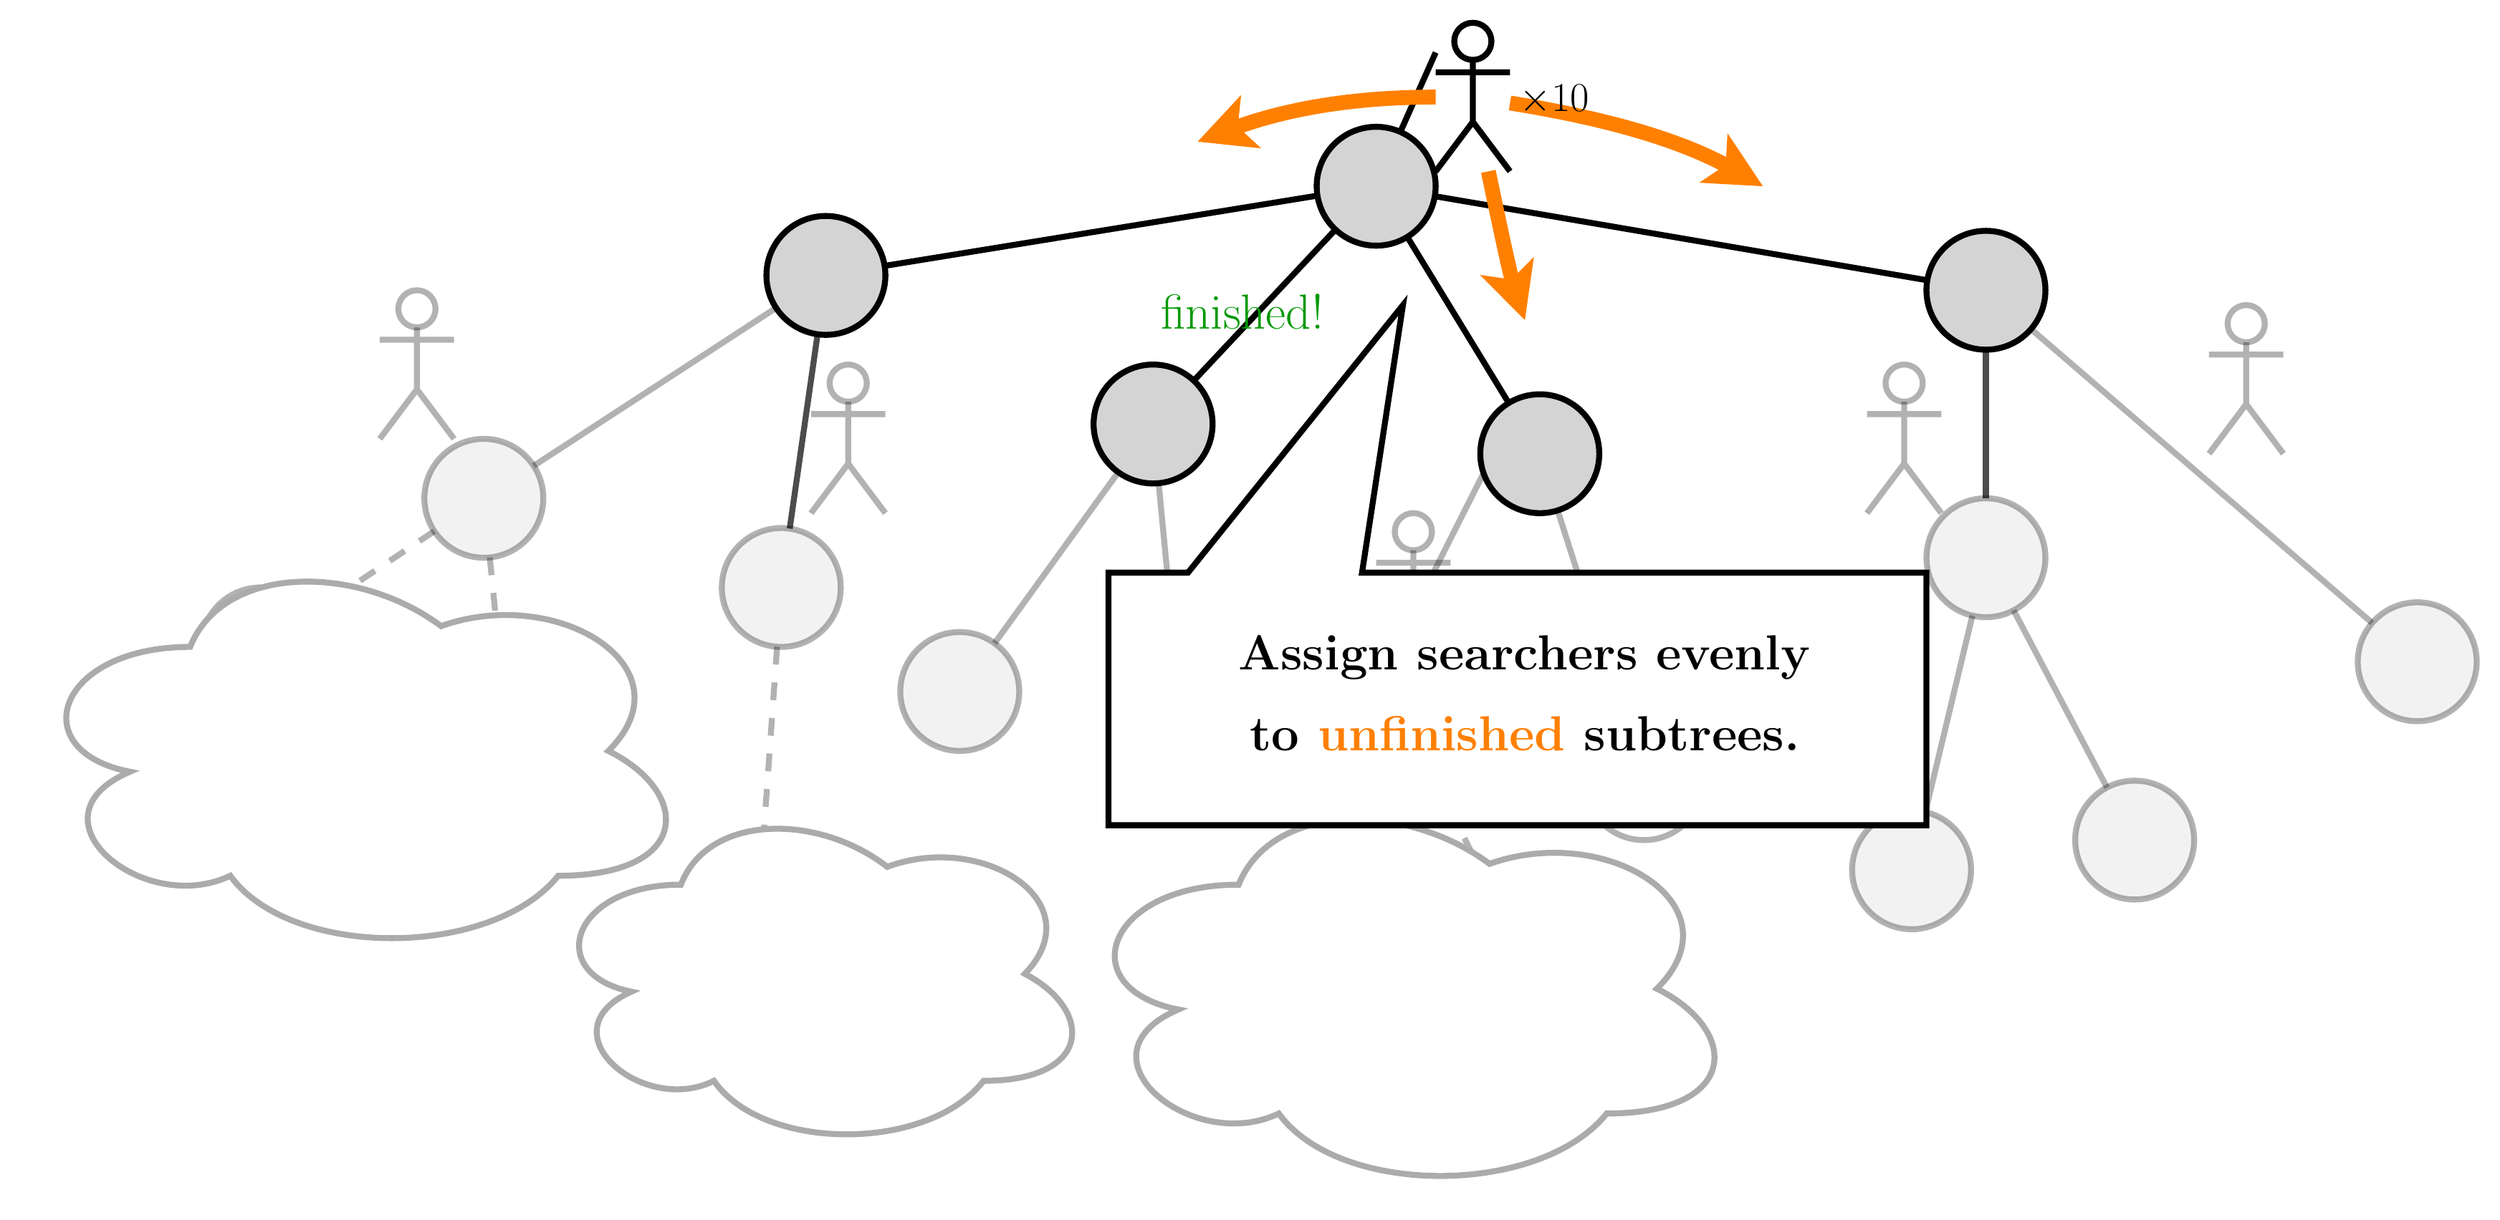
\begin{tikzpicture}[y=1pt, x=1pt, yscale=\globalscale,xscale=\globalscale, every node/.append style={scale=\globalscale}, inner sep=0pt, outer sep=0pt]
  \path[draw=black,line width=3.0pt,miter limit=10.0] (654.383, 507.495) -- (436.11, 472.05);



  \path[draw=black,line width=3.0pt,miter limit=10.0] (663.473, 490.373) -- (592.02, 414.135);



  \path[draw=black,line width=3.0pt,miter limit=10.0] (699.69, 486.683) -- (750.855, 402.847);



  \path[draw=black,line width=3.0pt,miter limit=10.0] (713.572, 507.217) -- (961.928, 464.798);



  \path[draw=black,line width=3.0pt,miter limit=10.0] (696.188, 539.663) -- (714.0, 579.75);



  \path[draw=black,fill=cd4d4d4,line width=3.0pt] (684.0, 512.25) ellipse (30.0pt and 30.0pt);



  \path[draw=black,draw opacity=0.3,line width=3.0pt,miter limit=10.0] (381.382, 450.847) -- (259.125, 371.138);



  \path[draw=black,draw opacity=0.7,line width=3.0pt,miter limit=10.0] (402.308, 437.543) -- (388.245, 339.45);



  \path[draw=black,fill=cd4d4d4,line width=3.0pt] (406.5, 467.25) ellipse (30.0pt and 30.0pt);



  \path[draw=black,draw opacity=0.3,line width=3.0pt,miter limit=10.0] (553.95, 367.92) -- (491.565, 281.572);



  \path[draw=black,draw opacity=0.3,line width=3.0pt,miter limit=10.0] (574.312, 362.385) -- (583.658, 264.615);



  \path[draw=black,fill=cd4d4d4,line width=3.0pt] (571.5, 392.25) ellipse (30.0pt and 30.0pt);



  \path[draw=black,draw opacity=0.3,line width=3.0pt,miter limit=10.0] (775.508, 348.638) -- (809.902, 240.84);



  \path[draw=black,draw opacity=0.3,line width=3.0pt,miter limit=10.0] (738.217, 367.545) -- (697.305, 286.335);



  \path[draw=black,fill=cd4d4d4,line width=3.0pt] (766.5, 377.25) ellipse (30.0pt and 30.0pt);



  \path[draw=black,draw opacity=0.3,line width=3.0pt,miter limit=10.0] (1014.232, 440.175) -- (1186.275, 291.84);



  \path[draw=black,draw opacity=0.7,line width=3.0pt,miter limit=10.0] (991.5, 429.75) -- (991.5, 354.75);



  \path[draw=black,fill=cd4d4d4,line width=3.0pt] (991.5, 459.75) ellipse (30.0pt and 30.0pt);



  \path[draw=black,draw opacity=0.3,line width=3.0pt,miter limit=10.0,dash pattern=on 9.0pt off 9.0pt] (209.003, 338.16) -- (146.46, 296.392);



  \path[draw=black,draw opacity=0.3,line width=3.0pt,miter limit=10.0,dash pattern=on 9.0pt off 9.0pt] (236.985, 324.9) -- (246.015, 234.6);



  \path[draw=black,fill=cd4d4d4,fill opacity=0.3,draw opacity=0.3,line width=3.0pt] (234.0, 354.75) ellipse (30.0pt and 30.0pt);



  \path[draw=black,fill=white,fill opacity=0.3,draw opacity=0.3,line width=3.0pt] (369.0, 99.75) ellipse (30.0pt and 30.0pt);



  \path[draw=black,draw opacity=0.3,line width=3.0pt,miter limit=10.0,dash pattern=on 9.0pt off 9.0pt] (381.878, 279.825) -- (371.138, 129.675);



  \path[draw=black,fill=cd4d4d4,fill opacity=0.3,draw opacity=0.3,line width=3.0pt] (384.0, 309.75) ellipse (30.0pt and 30.0pt);



  \path[draw=black,fill=cd4d4d4,fill opacity=0.3,draw opacity=0.3,line width=3.0pt] (474.0, 257.25) ellipse (30.0pt and 30.0pt);



  \path[draw=black,fill=white,fill opacity=0.3,draw opacity=0.3,line width=3.0pt] (586.5, 234.75) ellipse (30.0pt and 30.0pt);



  \path[draw=black,fill=white,fill opacity=0.3,draw opacity=0.3,line width=3.0pt] (819.0, 212.25) ellipse (30.0pt and 30.0pt);



  \path[draw=black,draw opacity=0.3,line width=3.0pt,miter limit=10.0] (690.428, 213.502) -- (662.618, 120.982);



  \path[draw=black,draw opacity=0.3,line width=3.0pt,miter limit=10.0,dash pattern=on 9.0pt off 9.0pt] (712.418, 215.415) -- (753.083, 134.085);



  \path[draw=black,fill=white,fill opacity=0.3,draw opacity=0.3,line width=3.0pt] (699.0, 242.25) ellipse (30.0pt and 30.0pt);



  \path[draw=black,fill=white,fill opacity=0.3,draw opacity=0.3,line width=3.0pt] (654.0, 92.25) ellipse (30.0pt and 30.0pt);



  \path[draw=black,fill=white,fill opacity=0.3,draw opacity=0.3,line width=3.0pt] (766.5, 107.25) ellipse (30.0pt and 30.0pt);



  \path[draw=black,fill=cd4d4d4,fill opacity=0.3,draw opacity=0.3,line width=3.0pt] (1209.0, 272.25) ellipse (30.0pt and 30.0pt);



  \path[draw=black,draw opacity=0.3,line width=3.0pt,miter limit=10.0] (1005.465, 298.2) -- (1052.527, 208.8);



  \path[draw=black,draw opacity=0.3,line width=3.0pt,miter limit=10.0] (984.668, 295.537) -- (960.945, 196.432);



  \path[draw=black,fill=cd4d4d4,fill opacity=0.3,draw opacity=0.3,line width=3.0pt] (991.5, 324.75) ellipse (30.0pt and 30.0pt);



  \path[draw=black,fill=cd4d4d4,fill opacity=0.3,draw opacity=0.3,line width=3.0pt] (1066.5, 182.25) ellipse (30.0pt and 30.0pt);



  \path[draw=black,fill=cd4d4d4,fill opacity=0.3,draw opacity=0.3,line width=3.0pt] (954.0, 167.25) ellipse (30.0pt and 30.0pt);



  \path[draw=black,fill=white,fill opacity=0.3,draw opacity=0.3,line width=3.0pt] (249.0, 204.75) ellipse (30.0pt and 30.0pt);



  \path[draw=black,fill=white,fill opacity=0.3,draw opacity=0.3,line width=3.0pt] (121.5, 279.75) ellipse (30.0pt and 30.0pt);



  \path[draw=cababab,fill=white,line width=3.0pt,miter limit=10.0] (614.625, 159.75).. controls (547.125, 159.75) and (530.25, 107.25) .. (584.25, 96.75).. controls (530.25, 73.65) and (591.0, 23.25) .. (634.875, 44.25).. controls (665.25, 2.25) and (766.5, 2.25) .. (800.25, 44.25).. controls (867.75, 44.25) and (867.75, 86.25) .. (825.562, 107.25).. controls (867.75, 149.25) and (800.25, 191.25) .. (741.188, 170.25).. controls (699.0, 201.75) and (631.5, 201.75) .. (614.625, 159.75) -- cycle;



  \path[draw=cababab,fill=white,line width=3.0pt,miter limit=10.0] (333.375, 159.75).. controls (277.875, 159.75) and (264.0, 114.75) .. (308.4, 105.75).. controls (264.0, 85.95) and (313.95, 42.75) .. (350.025, 60.75).. controls (375.0, 24.75) and (458.25, 24.75) .. (486.0, 60.75).. controls (541.5, 60.75) and (541.5, 96.75) .. (506.812, 114.75).. controls (541.5, 150.75) and (486.0, 186.75) .. (437.438, 168.75).. controls (402.75, 195.75) and (347.25, 195.75) .. (333.375, 159.75) -- cycle;



  \path[draw=cababab,fill=white,line width=3.0pt,miter limit=10.0] (85.875, 279.75).. controls (18.375, 279.75) and (1.5, 227.25) .. (55.5, 216.75).. controls (1.5, 193.65) and (62.25, 143.25) .. (106.125, 164.25).. controls (136.5, 122.25) and (237.75, 122.25) .. (271.5, 164.25).. controls (339.0, 164.25) and (339.0, 206.25) .. (296.812, 227.25).. controls (339.0, 269.25) and (271.5, 311.25) .. (212.438, 290.25).. controls (170.25, 321.75) and (102.75, 321.75) .. (85.875, 279.75) -- cycle;



  \path[draw=black,fill=white,fill opacity=0.3,draw opacity=0.3,line width=3.0pt] (200.25, 450.375) ellipse (9.375pt and 9.375pt);



  \path[draw=black,draw opacity=0.3,line width=3.0pt,miter limit=10.0] (200.25, 441.0) -- (200.25, 409.748)(200.25, 434.752) -- (181.5, 434.752)(200.25, 434.752) -- (219.0, 434.752)(200.25, 409.748) -- (181.5, 384.75)(200.25, 409.748) -- (219.0, 384.75);



  \path[draw=black,fill=white,fill opacity=0.3,draw opacity=0.3,line width=3.0pt] (417.75, 412.875) ellipse (9.375pt and 9.375pt);



  \path[draw=black,draw opacity=0.3,line width=3.0pt,miter limit=10.0] (417.75, 403.5) -- (417.75, 372.247)(417.75, 397.252) -- (399.0, 397.252)(417.75, 397.252) -- (436.5, 397.252)(417.75, 372.247) -- (399.0, 347.25)(417.75, 372.247) -- (436.5, 347.25);



  \path[draw=black,fill=white,fill opacity=0.3,draw opacity=0.3,line width=3.0pt] (702.75, 337.875) ellipse (9.375pt and 9.375pt);



  \path[draw=black,draw opacity=0.3,line width=3.0pt,miter limit=10.0] (702.75, 328.5) -- (702.75, 297.247)(702.75, 322.252) -- (684.0, 322.252)(702.75, 322.252) -- (721.5, 322.252)(702.75, 297.247) -- (684.0, 272.25)(702.75, 297.247) -- (721.5, 272.25);



  \path[draw=black,fill=white,fill opacity=0.3,draw opacity=0.3,line width=3.0pt] (950.25, 412.875) ellipse (9.375pt and 9.375pt);



  \path[draw=black,draw opacity=0.3,line width=3.0pt,miter limit=10.0] (950.25, 403.5) -- (950.25, 372.247)(950.25, 397.252) -- (931.5, 397.252)(950.25, 397.252) -- (969.0, 397.252)(950.25, 372.247) -- (931.5, 347.25)(950.25, 372.247) -- (969.0, 347.25);



  \path[draw=cff8000,line width=7.5pt,miter limit=10.0] (740.565, 519.75) .. controls (747.855, 484.75) and (752.168, 465.248) .. (753.503, 461.243);



  \path[draw=cff8000,fill=cff8000,line width=7.5pt,miter limit=10.0] (756.345, 452.707) -- (746.865, 462.195) -- (753.503, 461.243) -- (758.243, 465.99) -- cycle;



  \path[draw=cff8000,line width=7.5pt,miter limit=10.0] (751.5, 554.25) .. controls (801.5, 546.25) and (838.967, 535.125) .. (863.902, 520.875);



  \path[draw=cff8000,fill=cff8000,line width=7.5pt,miter limit=10.0] (871.717, 516.413) -- (858.323, 517.155) -- (863.902, 520.875) -- (864.277, 527.572) -- cycle;



  \path[draw=cff8000,line width=7.5pt,miter limit=10.0] (714.0, 557.25) .. controls (674.0, 557.25) and (639.425, 551.785) .. (610.275, 540.855);



  \path[draw=cff8000,fill=cff8000,line width=7.5pt,miter limit=10.0] (601.853, 537.697) -- (610.98, 547.523) -- (610.275, 540.855) -- (615.195, 536.288) -- cycle;



  \path[draw=black,fill=white,line width=3.0pt] (732.75, 585.375) ellipse (9.375pt and 9.375pt);



  \path[draw=black,line width=3.0pt,miter limit=10.0] (732.75, 576.0) -- (732.75, 544.747)(732.75, 569.753) -- (714.0, 569.753)(732.75, 569.753) -- (751.5, 569.753)(732.75, 544.747) -- (714.0, 519.75)(732.75, 544.747) -- (751.5, 519.75);



  \path (699.0, 576.0) rectangle (849.0, 538.5);



  \node[anchor=south] (text7441) at (774.0, 548.4){\fontsize{21.0pt}{25.2pt}\selectfont \(\times 10\)};



  \path (549.0, 474.75) rectangle (684.0, 429.75);



  \node[anchor=south] (text3132) at (616.5, 440.25){\fontsize{30.0pt}{36.0pt}\selectfont \textcolor[HTML]{009900}{finished!}};



  \path[draw=black,fill=white,fill opacity=0.3,draw opacity=0.3,line width=3.0pt] (1122.75, 442.875) ellipse (9.375pt and 9.375pt);



  \path[draw=black,draw opacity=0.3,line width=3.0pt,miter limit=10.0] (1122.75, 433.5) -- (1122.75, 402.247)(1122.75, 427.252) -- (1104.0, 427.252)(1122.75, 427.252) -- (1141.5, 427.252)(1122.75, 402.247) -- (1104.0, 377.25)(1122.75, 402.247) -- (1141.5, 377.25);



  \path[draw=black,fill=white,line width=3.0pt,miter limit=10.0,cm={ -1.0,0.0,-0.0,-1.0,(1510.5, 642.0)}] (549.0, 452.25) -- (961.5, 452.25) -- (961.5, 324.75) -- (921.375, 324.75) -- (813.0, 189.75) -- (833.625, 324.75) -- (549.0, 324.75) -- cycle;



  \path (571.5, 298.5) rectangle (946.5, 216.0);



  \node[anchor=south] (text7035) at (759.0, 263.25){\fontsize{30.0pt}{36.0pt}\selectfont \textbf{Assign searchers evenly}};



  \node[anchor=south] (text2379) at (759.0, 227.25){\fontsize{30.0pt}{36.0pt}\selectfont \textbf{to \textcolor[HTML]{FF8000}{unfinished} subtrees.}};




\end{tikzpicture}
